\section{Instancias de pruebas}\label{sect:busquedas}
En esta sección se presentan las consultas que se utilizaron para evaluar las propuestas algorítmicas presentadas en este trabajo. Las consultas se hicieron sobre dos bases de datos. Una de ellas corresponde a la base de datos de artículos provista por \textit{\textquotedblleft A Data-Driven Journey through Software Engineering Research\textquotedblright}\cite{dataDrive}. La otra base de datos corresponde a atracciones turísticas de Europa. A continuación se describe para cada consulta de cada base da datos la función de similitud, el atributo de complementariedad y el presupuesto. 

\subsection{Base de datos de artículos}
La base de datos utilizada es la proporcionada por \textit{\textquotedblleft A Data-Driven Journey through Software Engineering Research\textquotedblright}\cite{dataDrive}. La misma contiene unos $7800$ artículos relacionados con la ingeniería de software presentados en diferentes conferencias entre los años 1975 y 2011 catalogados por autores, tópicos relevantes, conferencia donde fue presentado el trabajo y afiliaciones. Además cada artículo tiene asociado un \texttt{topicProfile} de los autores, que expresa el porcentaje de la relevancia de cada tópico considerado dentro del artículo. Este valor fue calculado en función de los temas de las conferencias o revistas de los trabajos citados en el artículo. La base considera 37 tópicos para definir el \texttt{topicProfile}. De los $9800$ autores se tiene la información de la universidad a la que cada uno pertenece y la región donde se encuentra dicha universidad.

El \texttt{topicProfile} es lo que permitirá definir la similitud, no sólo entre los artículos, sino también entre los autores y las universidades de la base de datos de una manera prácticamente directa.

Los criterios de las búsquedas realizadas sobre la base de datos se concibieron a partir de lo que se considera que es de interés general. Por ejemplo, una posible consulta sobre esta base de datos podría ser la búsqueda de artículos sobre núcleos temáticos característicos en las distintas conferencias, de manera que observando un paquete se podría conocer qué se dice sobre este tema en cada una de las conferencias. En otro escenario, con el propósito de armar paneles de expertos, puede resultar de interés la búsqueda de investigadores que trabajan en tópicos similares con afiliación en distintas universidades. También se puede querer conocer universidades de distintas regiones con grupos de investigación trabajando en tópicos similares.

Por lo establecido en \cite{compositeRetrival} para las búsquedas se deben realizar las siguientes definiciones:
\begin{itemize}
  \item \textbf{Similitud}: Función que dado dos ítems devuelve la similitud entre estos.
  \item \textbf{Costo}: Función que dado un ítem devuelve el costo del mismo.
  \item \textbf{Presupuesto}: El presupuesto que se tiene, el cual no podrá ser excedido por ningún paquete.
  \item \textbf{Complementariedad}: Propiedad del ítem que es único en cada paquete.
\end{itemize}

Para todas las búsquedas, sin importar el ítem que sea (artículo, autor o universidad), se definió que el costo de cada ítem sea de una unidad y que el presupuesto para cada búsqueda sea de cinco unidades. En consecuencia, todos los paquetes de todos los resultados contienen como máximo cinco ítems. Se tomó esta decisión para que cada paquete contenga como máximo un número fijo de elementos. Además se estableció que sean diez los paquetes devueltos en cada búsqueda. El motivo para tomar esta decisión es que un humano pueda valorizar el resultado propuesto fácilmente. Entonces, de aquí en adelante, para cada criterio de búsqueda se deben definir únicamente la función de similitud y la propiedad de complementariedad.

Como se mencionó anteriormente, en la base de datos cada artículo cuenta con su \texttt{Topic Profile}. El \texttt{Topic Profile} define el perfil de un artículo asignándole un porcentaje a cada tópico que se hace referencia. En el caso del artículo \texttt{A Cognitive-Based Mechanism for Constructing Software Inspection Teams} el \texttt{Topic Profile} se compone por los tópicos  REQUIREMENTS, RELIABILITY, TESTING y SOFTWARE QUALITY. El porcentaje de cada uno de estos es 71.43 \%, 17.86 \%, 7.14 \% y 3.57 \% respectivamente. Esto significa que el 71.43\% de los trabajos citados en este artículo fueron presentados en conferencias o publicados en revistas vinculadas al área REQUIREMENTS.

El modelo computacional del perfil de cada artículo es un vector que la dimensión corresponde a la cantidad de tópicos y cada posición representa un tópico diferente. El valor de cada posición del vector es el porcentaje del tópico que le corresponde a ese artículo según el \textit{Topic Profile} de la base de datos. Más adelante se explica como estos vectores se utilizan para comparar la similitud entre los artículos.

Para los autores no se cuenta con información más allá de los artículos que escribieron, pero sólo con eso alcanza para poder generar un perfil de autores. Para cada autor se hace la suma vectorial de cada uno de los \texttt{Topic Profile} de los artículos en los cuales participó y con eso se obtiene el \texttt{Topic Profile de Autores}. Para obtener el perfil de las universidades se aplicó el mismo criterio. Se realiza la suma vectorial de cada uno de los \texttt{Topic Profile de Autores} pertenecientes a la misma universidad y así se genera el \texttt{Topic Profile de Universidades}. En ambos casos se aplica la normalización sobre los vectores resultantes.

Para clarificar mostramos un ejemplo de los perfiles de los elementos:

\begin{table}[H]
\begin{tabular}{lll}
	Artículo & Topic Profile & Autores \\
	Artículo 1 & $[$0.20, 0.40, 0.40, 0.00$]$ & Autor 1, Autor 2, Autor 3 \\
	Artículo 2 & $[$0.30, 0.70, 0.00, 0.00$]$ & Autor 2, Autor 3 \\
	Artículo 3 & $[$0.00, 0.10, 0.00, 0.90$]$ & Autor 2 \\
	Artículo 4 & $[$0.00, 0.00, 1.00, 0.00$]$ & Autor 1, Autor 3 \\
\end{tabular}
\label{tabla:topicProfileEj1}
\end{table}

\begin{table}[H]
\begin{tabular}{lll}
	Autor & Topic Profile & Universidad \\
	Autor 1 & $[$0.14, 0.27, 0.95, 0.00$]$ & Universidad 1 \\
	Autor 2 & $[$0.30, 0.74, 0.25, 0.55$]$ & Universidad 2 \\
	Autor 3 & $[$0.27, 0.60, 0.76, 0.0$]$ & Universidad 2 \\
\end{tabular}
\label{tabla:topicProfileEj2}
\end{table}

\begin{table}[H]
\begin{tabular}{ll}
	Universidad & Topic Profile \\
	Universidad 1 & $[$0.14, 0.27, 0.95, 0.00$]$ \\
	Universidad 2 & $[$0.31, 0.72, 0.54, 0.30$]$ \\
\end{tabular}
\label{tabla:topicProfileEj3}
\end{table}

Para la evaluación las consultas realizadas son:
\begin{enumerate}
	\item
		Artículos con tópicos similares presentados en distintas conferencias.
		\begin{itemize}
			\item \textbf{Similitud}: Función que compara el perfil de cada artículo.
			\item \textbf{Complementariedad}: Lugar dónde fue presentado.
		\end{itemize}

	\item
	Autores que escribieron artículos con tópicos similares afiliados a universidades distintas.
	\begin{itemize}
		\item \textbf{Similitud}: Función que compara el perfil de los autores.
		\item \textbf{Complementariedad}: Universidad de pertenencia del autor.
	\end{itemize}

	\item 
	Universidades en donde se escribieron artículos de tópicos similares que se encuentran en distintas regiones. 
	\begin{itemize}
		\item \textbf{Similitud}: Función que compara el perfil de las universidades.
		\item \textbf{Complementariedad}: Región de la institución.
	\end{itemize}
\end {enumerate}

Para obtener resultados de mayor calidad, se depuró de la base de datos aquellos artículos que no contengan la información del autor, de los tópicos (\textbf{topic profile}) o del lugar de publicación (\textbf{venue}). Quedando, luego de la depuración, $5500$ artículos.  

\paragraph{Función de similitud}
La similitud se emplea para comparar dos objetos y determinar qué tan parecido son entre si. En este trabajo definimos la similitud entre los objetos de la base de datos de artículos mediante la \textbf{similitud coseno}. Esta es una medida de similitud entre dos vectores en un espacio vectorial provisto de un producto escalar que mide el coseno del ángulo comprendido entre ellos.

Entonces se define la función de similitud $S(U_i, V_j)$ para los vectores $U_i$ y $V_j$ a partir del producto escalar\\

\begin{equation} \label{eq:angulovectorial}
\cos(\theta) =  \dfrac{\overrightarrow{U_i} . \overrightarrow{V_j}}{\overrightarrow{\lVert U_i\lVert}.\overrightarrow{\lVert V_j\lVert}}
\end{equation}

Para esta instancia los objetos (ahora artículos, autores o universidades) están representados por vectores, donde cada dimensión corresponde a un tópico cuyo valor se corresponde con el valor del tópico del objeto según la base de datos \cite{dataDrive}. Por lo tanto el objeto $a$ se representa con el vector $V_a = [v_1,v_2,...,v_3]$ que cumple con las siguientes propiedades:
\begin{enumerate}
 \item $v_i \geq 0$
 \item $\sum{v_i} = 1$
\end{enumerate}

Como los componentes de todos los vectores son mayor o igual a cero se obtiene que $0\leq\cos(\theta)\leq1$, que implica que $S(V_i, V_j) \in \left[0, 1\right]$.

\begin{figure}[H]
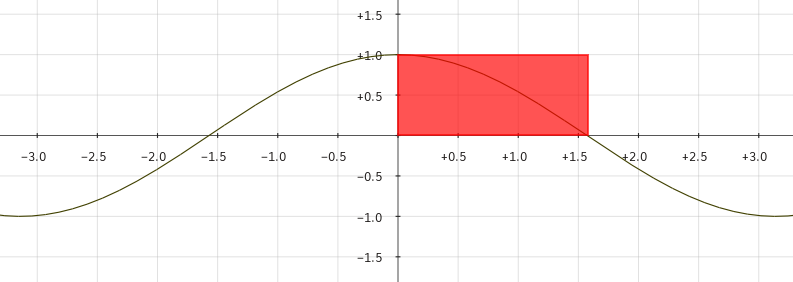
\includegraphics[width=0.8\textwidth]{img/coseno.png}
\caption{Comportamiento de la función $\cos$. En rojo la región que pertenece a la función de similitud}
\label{bus:img-coseno}
\end{figure}

%Para \textbf{similitud coseno} dos vectores proporcionales con la misma dirección la similitud es 1 (ya que es 0 el ángulo que se forma). Por lo que esta similitud no diferencia entre un artículo profesional y un artículo de un diario que cubre el mismo tópico. Por ejemplo si dos artículos que cubren un mismo y único tópico, pero para uno el valor del tópic Esta debilidad de la medida basada en el ángulo no interfiere en este trabajo por la segunda propiedad de los vectores del problema, porque para que dos vectores sean proporcionalmente iguales tienen que ser idénticos y en tal caso es correcto que la similitud entre ellos sea 1.

Con el objetivo de simplificar la ejecución de los algoritmos, considerando que el costo de calcular $cos()$ de los vectores es alto, se decidió realizar el cáculo de la similitud de los artículos, autores y universidades previamente a la ejecución de los algoritmos de búsquedas

\subsection{Base de dato de atracciones turísticas}
Se utilizó una instancia de datos correspondiente a 200 atracciones turísticas de Europa, con datos relevados del sitio \textit{TripAdvisor}. De cada atracción se tiene la información del precio, del tipo (parque, museo, edificio) y de la distancia geográfica con el resto de las atracciones.

El propósito de la búsqueda es darle al usuario distintas opciones de circuitos turísticos que contienen atracciones, con las siguientes requerimientos: evitar realizar largos traslados; que haya variedad en el tipo de atracción y que que el costo del circuito no supere el presupuesto del turista. Por lo tanto el modelo de la búsqueda quedo diseñada de la siguiente manera:

\begin{itemize}
	\item \textbf{Similitud}: La inversa de la distancia entre las atracciones. 
	\item \textbf{Costo}: Precio de la atracción. 
	\item \textbf{Presupuesto}: Presupuesto del turista. 
	\item \textbf{Complementariedad}: Tipo de atracción.
\end{itemize}

\section{Análisis de resutados}\label{sect:resultados}

Para la experimentación se utilizó una máquina Desktop Intel(R) Core(TM) i5-4570T CPU @ 2.90GHz, 5.7G Ram, con DB: 5.5.46-MariaDB-1ubuntu0.14.04.2.

El análisis que se realiza de los resultados obtenidos es comparando la calidad de los resultados de los algoritmos discutidos en \autoref{chap:nuevas-propuestas}, sobre las bases de datos de \autoref{sect:busquedas}. Con el objetivo de evaluar las propuestas algorítmicas, se consideraron los siguientes métodos:

\begin{itemize}
\item{$alg1$} PAC(C-HAC / selección simple)
\item{$alg2$} PAC(BOBO-10 / selección simple)
\item{$alg3$} PAC(BOBO-10 / selección proporcional)
\item{$alg4$} PAC(BOBO-10 / selección proporcional) + tabú
\item{$alg5$} PAC(Intra-Inter C-HAC / selección proporcional)
\item{$alg6$} PAC(Intra-Inter C-HAC / selección proporcional) + tabú
\item{$alg7$} Construcción golosa
\item{$alg8$} Construcción golosa + tabú
\end{itemize}

Tanto $alg1$ como $alg2$ corresponden a las metodologías propuestas en \cite{compositeRetrival}. Los demás algoritmos involucran las mejoras propuestas en este trabajo. En el caso de PAC es \texttt{Intra-Inter C-HAC} en la etapa de producción y la selección proporcional en la etapa de selección, además de la introducción de búsquedas tabú. En \texttt{PAC}, la búsqueda tabú \texttt{Inter-Paquete} se realiza al finalizar la etapa de producción y la \texttt{Intra-Paquete} luego de la selección. En la \texttt{Búsqueda Golosa} a la solución obtenida se realiza la búsqueda tabú \texttt{Intra-Paquete}. Cabe señalar que no se tienen en consideración BOBO-Ex y CAP ya que para el tamaño de la instancia los tiempos de ejecución de esos algoritmos resultaron prohibitivos. A partir de experimentación preliminar con BOBO para valores $c=1, 5$ y $10$, resultó $c=10$ la opción más competitiva. Para la búsquedas tabú se definió que la cantidad de iteraciones de permanencia de un elemento en la lista tabú sea el promedio de elementos que tiene un paquete en la solución inicial.

Para realizar una comparación entre la calidad de las soluciones obtenidas por los diferentes algoritmos, se ha evaluado para los $\gamma \in \left\{0,1; 0,3; 0,4; 0,5; 0,6; 0,7; 0,8; 0,9\right\} $el porcentaje de deterioro de cada solución.

En el caso de la búsqueda de artículos, que es el escenario que contiene la mayor cantidad de objetos, los tiempos de ejecución  para los algoritmos C-HAC ($alg1$, $algo5$ y $alg6$) son del orden de los 5 minutos, mientras que para los algoritmos BOBO ($alg2$, $alg3$ y $alg4$) de 2 minutos y los golosos ($alg7$ y $alg8$) de los x minutos. Los incrementos de tiempo debido a la ejecución de las metaheruísticas de mejora son despreciables, están entre los 5 y 7 segundos. Por lo cual no se considera que el tiempo sea un factor que valga la pena analizar.

\subsection{Base de datos de artículos}
Para comprender el comportamiento de los resultados de las búsquedas se diseñaron dos tipos de gráficos que permiten visualizar la cohesión de los paquetes y la distancia entre ellos. De esta forma se podrá analizar la calidad del resultado obtenido más allá del valor de la función objetivo.

Los gráficos del estilo de la figura \ref{res:img-explain-bars} permiten analizar la distribución de los tópicos de una solución a nivel de paquete y de la relación con otros. Las filas corresponden a los 10 paquetes obtenidos y las columnas a los 38 tópicos considerados. El tamaño del círculo representa la proporción del tópico en el perfil del artículo y el color hace referencia al paquete al cual artículo pertenece. Por lo tanto, dos artículos tendrán gran similitud cuando los patrones de sus círculos coincidan, tanto en tamaño como en distribución. Si para un paquete la distribución entre los tópicos y el tamaño de los círculos es similar entre sus artículos se puede deducir que este paquete es cohesivo (tiene buen valor intra). Por otro lado, si los patrones de los círculos de los dos artículos más similares entre distintos paquetes no coinciden, esto indica que el resultado es diverso.
\begin{figure}[H]
  \centering
    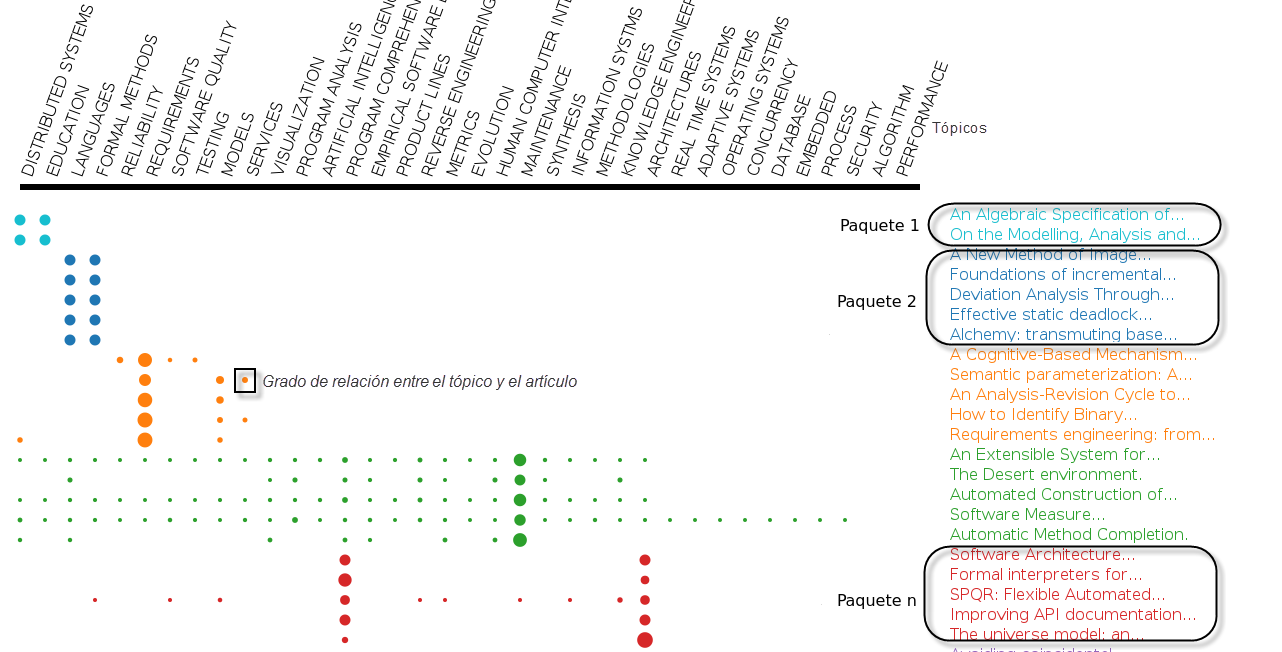
\includegraphics[width=1\textwidth]{img/explain-bars.png}
  \caption{}
  \label{res:img-explain-bars}
\end{figure}

Los gráficos de tipo burbuja de la figura \ref{res:img-explain-bubbles} son útiles para concluir el nivel de acoplamiento entre los paquetes de una solución, observando la relación entre los tópicos y los paquetes. Cada burbuja representa un tópico que contiene círculos; cada circulo es un artículo donde el tamaño es la proporción del articulo con el tópico y el color el paquete al que pertenece. Entonces si las burbujas contienen círculos de más de un color se puede decir que ese resultado no es muy diverso, mientras que el color de los círculos de las burbujas sea más homogéneo el resultado es más diverso. En cuanto a la cohesión de los paquetes, es más cohesivo cuando el tamaño de cada circulo dentro de cada burbuja sea similar (para el mismo color) y la distribución de los círculos entre cada burbuja es equitativa.

\begin{figure}[H]
  \centering
    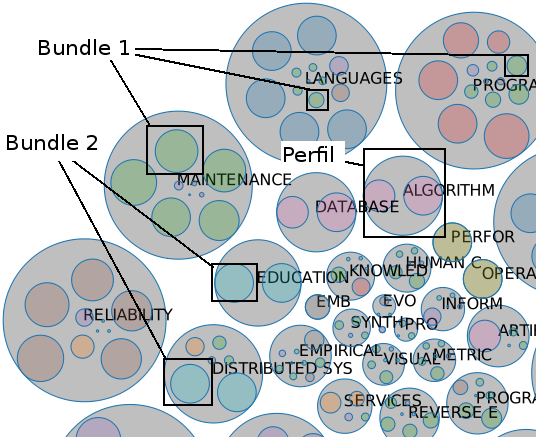
\includegraphics[width=0.5\textwidth]{img/explain-bubbles.png}
  \caption{}
  \label{res:img-explain-bubbles}
\end{figure}

\subsubsection{Búsqueda de artículos}
Para la búsqueda de artículos con tópicos similares en la tabla \ref{tabla:comp1} se observa los porcentajes de deterioro de cada solución respecto de la mejor solución obtenida por alguno de los ocho algoritmos. Una primera observación es que los algoritmos  Intra-Inter C-HAC reflejan el efecto buscado: a menores valores de $\gamma$ donde el valor inter tiene mayor peso, se obtienen mejores soluciones. Es decir, haber considerado en el proceso de generación de paquetes la funcion Intra-Inter benefició a la calidad de las soluciones obtenidas. Los algoritmos BOBO, no obtienen soluciones de la calidad de los algoritmos C-HAC y el proceso de selección proporcional no logra una mejora consistente para todos los valores de $\gamma$. Las soluciones obtenidas con el algoritmo de construcción golosa, no alcanzaron a mejorar las soluciones de C-HAC pero fueron ampliamente mejores que las de BOBO. En promedio el porcentaje de deterioro de BOBO fue de un $50\%$ mientras que el goloso fue de un $12\%$. 

Cabe resaltar el muy buen rendimiento de la búsqueda tabú, tanto en escenarios donde la solución inicial no es de buena calidad (algoritmo BOBO) así como también considerando soluciones de mejor calidad (algoritmo Intra-Inter C-HAC). En el primer caso, se obtienen porcentajes de mejora por encima del $70\%$. En el segundo caso, para varios valores de $\gamma$ la solución obtenida por la búsqueda tabú resultó ser la mejor opción y en otros con deterioros inferiores al $0.5\%$.

\begin{table}[H]
\begin{center}
\begin{tabular}{|c|c|c|c|c|c|c|c|c|}
\hline
$\gamma$&$alg1$&$alg2$&$alg3$&$alg4$&$alg5$&$alg6$&$alg7$&$alg8$ \\ \hline
0.1 & -2.05 & -32.70 & -36.18 & -7.45 & -0.42 & 0.00 & -4.53 & -3.53 \\
0.2 & -2.11 & -38.06 & -41.19 & -8.23 & 0.00 & 0.00 & -4.92 & -3.85 \\
0.3 & -2.31 & -45.21 & -47.35 & -8.01 & 0.00 & 0.00 & -9.17 & -7.66 \\
0.4 & -0.14 & -49.08 & -51.22 & -15.51 & 0.00 & 0.00 & -10.40 & -9.35 \\
0.5 & 0.00 & -52.35 & -54.23 & -17.87 & -0.31 & -0.31 & -12.97 & -10.38 \\
0.6 & 0.00 & -55.16 & -56.04 & -14.43 & -0.05 & -0.05 & -14.78 & -13.69 \\
0.7 & 0.00 & -56.88 & -56.57 & -17.02 & -0.41 & -0.41 & -16.21 & -15.08 \\
0.8 & 0.00 & -57.86 & -57.86 & -16.11 & -0.56 & -0.30 & -18.10 & -17.60 \\
0.9 & 0.00 & -58.92 & -58.92 & -15.91 & -0.48 & -0.35 & -20.47 & -17.61 \\ \hline 
\end{tabular}
\caption{Comparación de calidad de soluciones entre algoritmos} 
\label{tabla:comp1}
\end{center}
\end{table}

Al comparar las soluciones con mayor y menor función objetivo para los $\gamma = 0,1$ y $\gamma = 0,9$ se observa, en la figura \ref{res:comp1}, que para $\gamma = 0,1$ los tópicos (representados por burbujas) para la solución de \textit{alg 3} están presentes en varios paquetes (representados por círculos de colores) mientras que para el $alg6$ la mayoría de las burbujas contiene círculos de un solo color. De esta manera se visualiza que la solución de $alg6$ es más diversa. En $\gamma = 0,9$ el resultado obtenido con $alg3$ no se visualiza que cada burbuja contenga cinco circulos del mismo color, en cambio para la solución de $alg1$ si. Eso significa que los paquetes de la solución de $alg1$ son más cohesivos, ya que los cinco elementos de cada paquete tienen los mismos tópicos.

\begin{figure}[H]
	\centering
	\begin{tabular}{cc}
		$alg3$ & $alg6$\\
		\multicolumn{2}{c}{$\gamma=0.1$}\\ 
			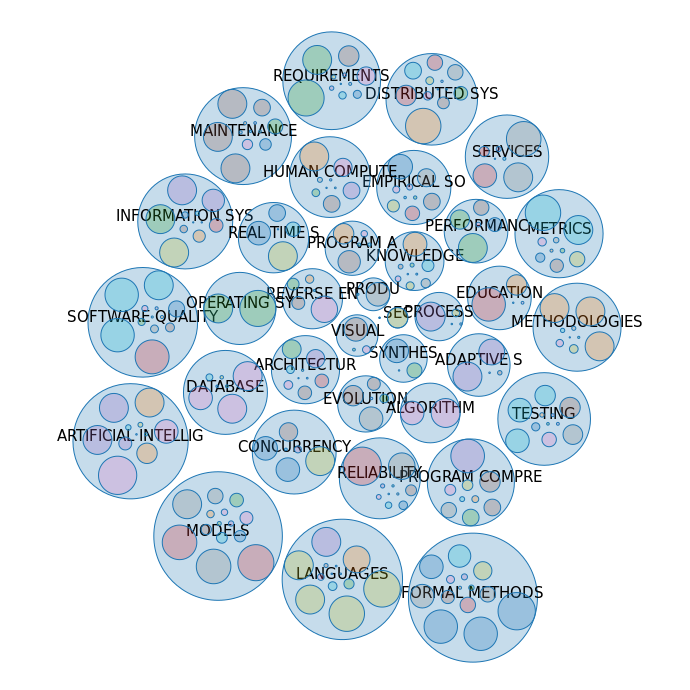
\includegraphics[width=0.5\linewidth]{img/gamma-01-burbujas-alg-3.png}&
			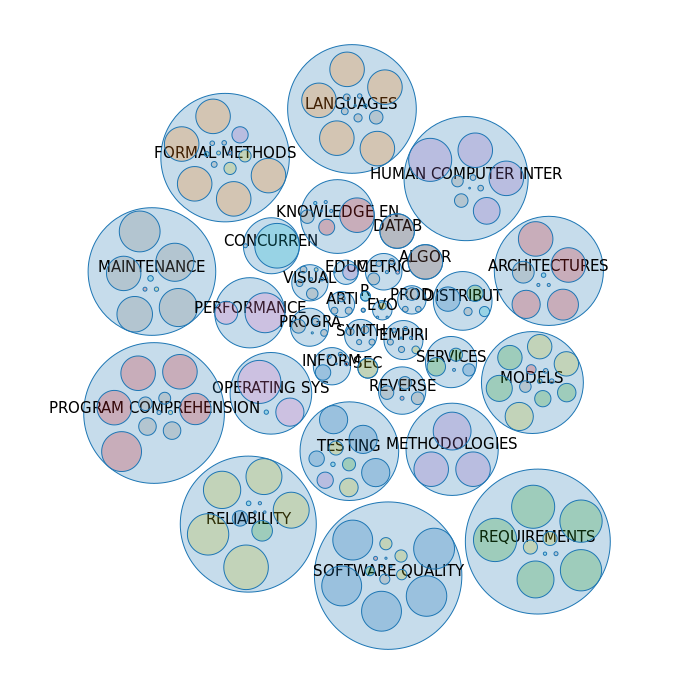
\includegraphics[width=0.5\linewidth]{img/gamma-01-burbujas-alg-6.png} 		\vspace{1cm}\\
			$alg3$ & $alg1$\\
		\multicolumn{2}{c}{$\gamma=0.9$}\\
			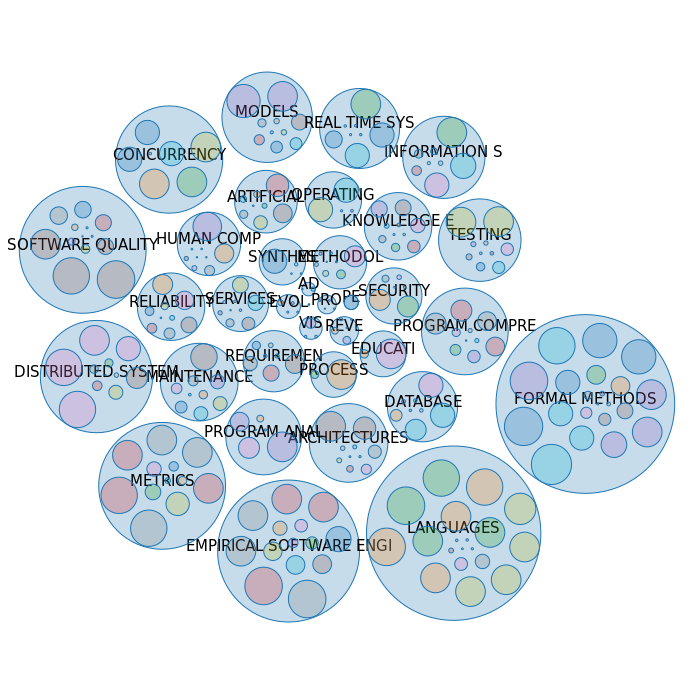
\includegraphics[width=0.5\linewidth]{img/gamma-09-burbujas-alg-3.png}&
			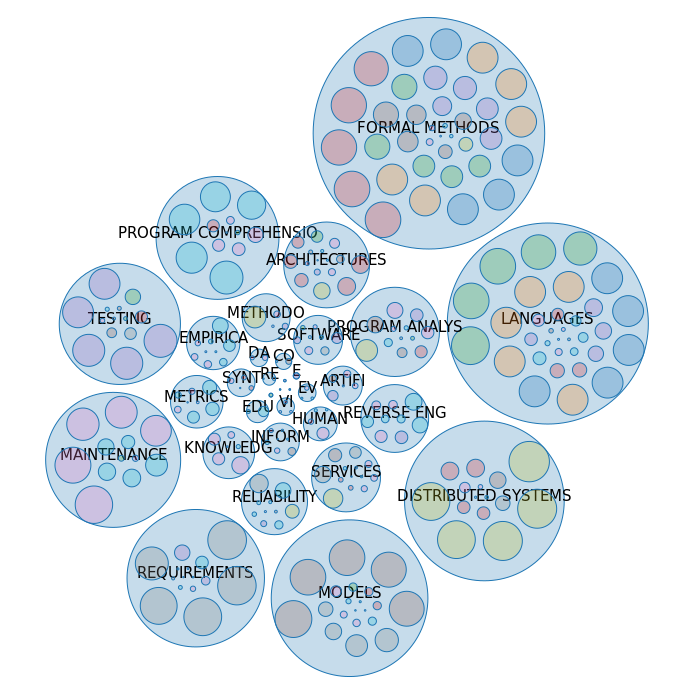
\includegraphics[width=0.5\linewidth]{img/gamma-09-burbujas-alg-1.png}\\
	\end{tabular}
	\caption{Comparación entre las soluciones con menor(izq) y mayor(der) función objetivos  para $\gamma\ 0,1\ y\ 0,9$}
	\label{res:comp1}
\end{figure}

La búsqueda tabú tiene su mayor impacto cuando es aplicada a la solución brindada por el algoritmo $alg3$ y en este contexto resulta una buena alternativa por su bajo costo computacional. En la Figura~\ref{res:bobo} se observa que para $\gamma=0.1$, la solución dada por el $alg3$ tiene artículos de distintos paquetes con patrones muy similares indicando un bajo valor inter-paquete. Por el contrario, luego de aplicar la búsqueda tabú los patrones de los artículos más similares entre distintos paquetes se volvieron más dispares, demostrando el aumento de la diversidad entre paquetes. Para $\gamma=0.9$, como puede observarse en la misma Figura~\ref{res:bobo}, en la solución brindada por el $alg4$ todos los paquetes tienen al menos un artículo cuyo patrón consiste en muchos círculos pequeños distribuidos en la mayoría de los tópicos en contraposición al resto de los artículos del mismo paquete con pocos círculos de gran tamaño, demostrando un bajo valor intra-paquete. En contraposición a los paquetes obtenidos luego de aplicar la búsqueda tabú, los cuáles son mucho más cohesivos. La última afirmación puede observarse en los círculos de los artículos dentro de un mismo paquete, quienes siguen patrones mucho más parecidos. Se puede afirmar que la búsqueda tabú es capaz de mejorar las características de la solución en función del parámetro $\gamma$.

Como se mencionó anteriormente, el algoritmo $C-HAC$ de \cite{compositeRetrival} ($alg1$) utiliza la función $Score$ para decidir el par de {\em clusters} a unir en la etapa de producción de paquetes y en la selección simple en la segunda fase. Estos dos criterios omiten la diversidad de los paquetes. De acuerdo a los resultados de la tabla \ref{tabla:comp1}, se pudo concluir que haber considerado la función Intra-Inter y la selección proporcional benefició la calidad de las soluciones cuando la misma es medida a partir de la función objetivo $w(S)$. Con el fin de evaluar que el $alg5$ es capaz de captar efectivamente la diversidad en la solución, se analiza las soluciones para $\gamma=0.5$. En este caso el $alg1$ obtuvo un valor de $intra=93,82$ y de $inter=35,49$, mientras que el $alg5$ logró valores de $intra=92,94$ y de $inter=35,96$. A pesar de que la solución de $alg1$ es levemente superior, la solución del $alg5$ aumentó el valor $inter$ el $1,32\%$ con un deterioro del valor $intra$ del $0,93\%$. Observando la Figura~\ref{res:comp1} se puede ver que la cohesión intra-paquete de ambas soluciones es equivalente. Sin embargo, la diversidad en la segunda solución es mayor, ya que los patrones entre los artículos más similares de distintos paquetes son más heterogéneos. 

\begin{figure}[H]
	\centering
	\begin{tabular}{cc}
		$alg3$ & $alg4$\\
		\multicolumn{2}{c}{$\gamma=0.1$}\\
			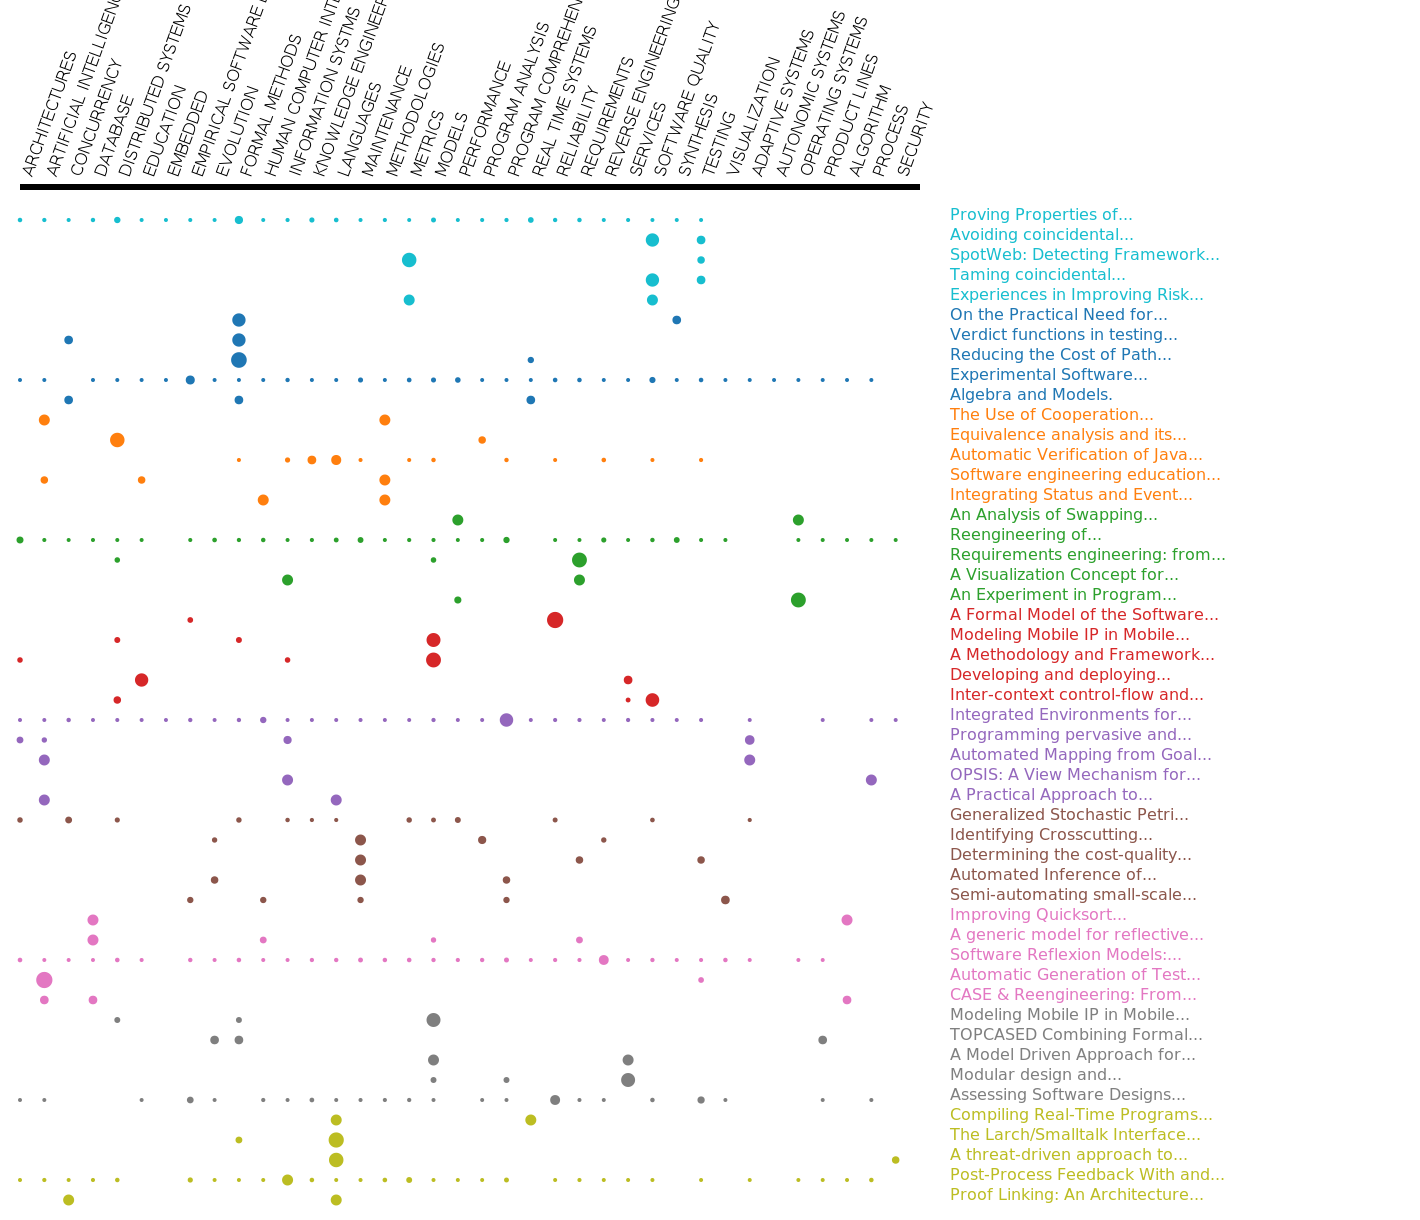
\includegraphics[width=0.5\linewidth]{img/gamma-01-alg-3.png}&
			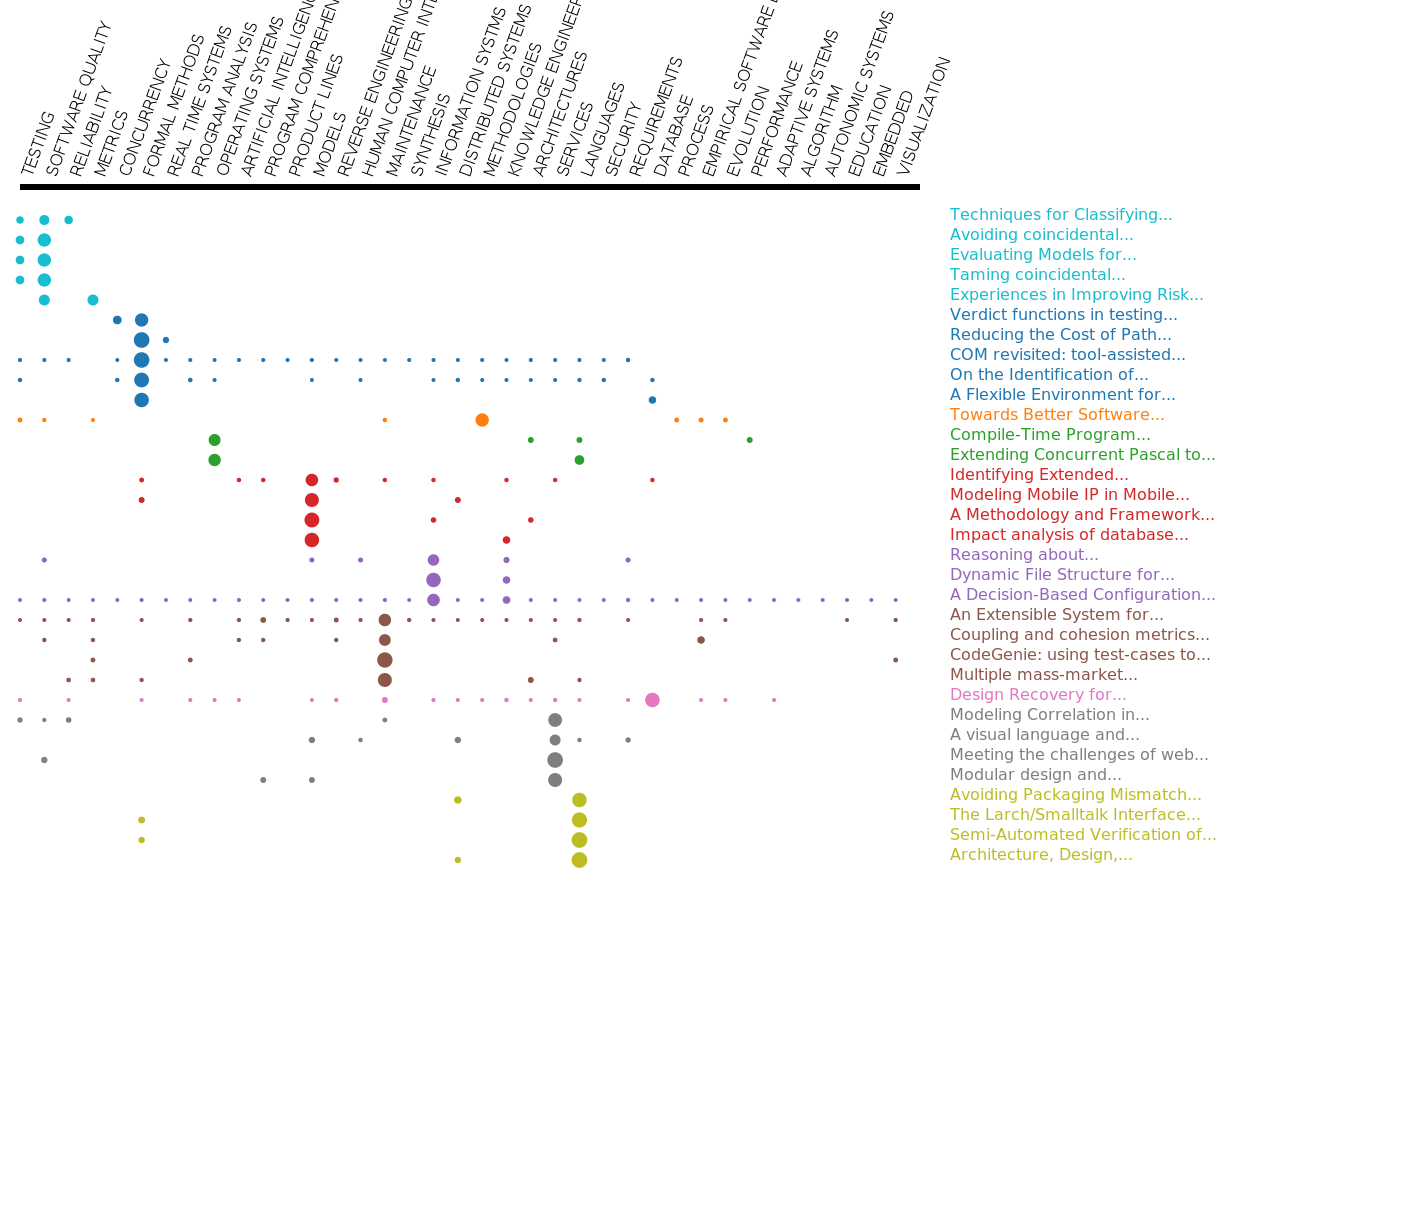
\includegraphics[width=0.5\linewidth]{img/gamma-01-alg-4.png} 		\vspace{1cm}\\
		\multicolumn{2}{c}{$\gamma=0.9$}\\
			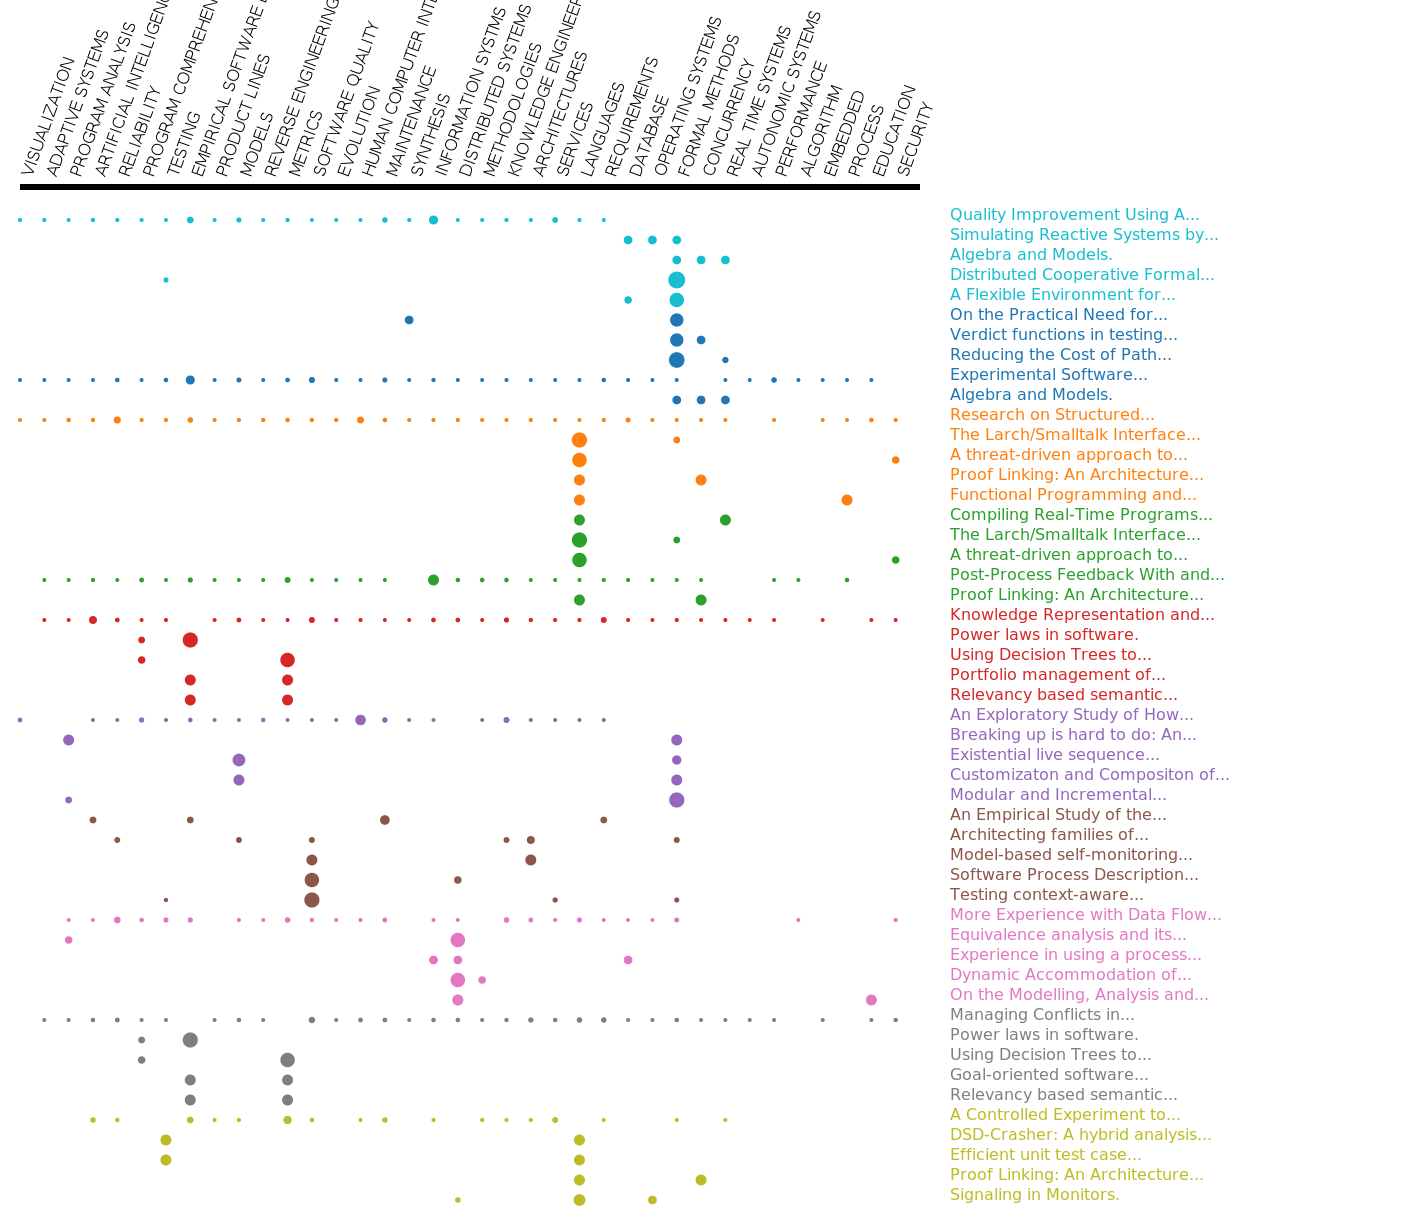
\includegraphics[width=0.5\linewidth]{img/gamma-09-alg-3.png}&
			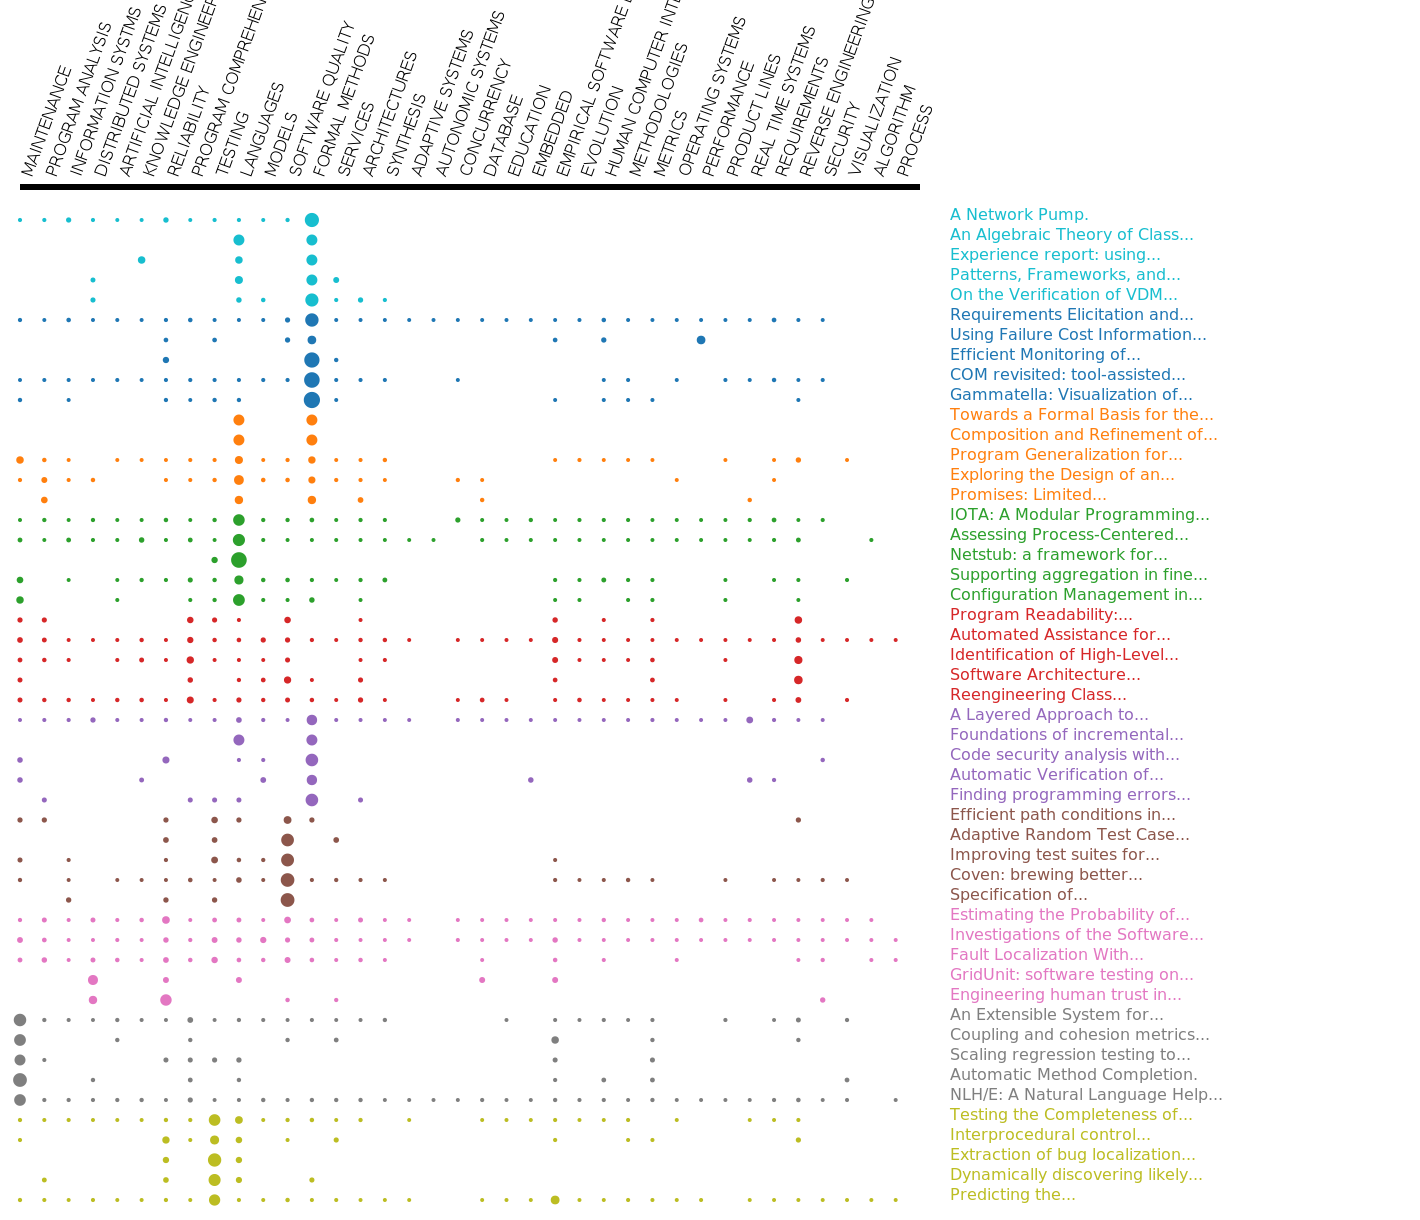
\includegraphics[width=0.5\linewidth]{img/gamma-09-alg-4.png}\\
	\end{tabular}
	\caption{Comparación de soluciones para BOBO-10 con y sin heurística de mejoramiento}
	\label{res:bobo}
\end{figure}

La decisión acerca del valor de $\gamma$ para priorizar un objetivo sobre el otro es realizada por el usuario. Una curva de frontera eficiente podría ayudar para examinar el balance (trade-off) entre los dos objetivos. La intención es que el usuario pueda analizar si una mejora significativa en el valor intra-paquete implica una degradación sustancial en el valor inter-paquetes y viceversa. Para ilustrar este análisis se presenta la Figura \ref{res:inter_intra}  que al comprar las soluciones obtenidas por los algoritmos $alg1$ y $alg5$ variando en pasos de $0,1$. Se observa que las soluciones provistas por $alg5$ no superan en todos los casos el inter en las soluciones obtenidas con $alg1$. En promedio el inter de las soluciones de $alg1$ superan a las de $alg5$ en un $0,65\%$. 

En la misma figura se compara las soluciones obtenidas por el algoritmo goloso $alg7$, que en promedio supera a las soluciones provistas por $alg2$ en $76\%$. De la comparación, se destaca que el valor de $\gamma$ impacta más en las soluciones de $alg2$.  

\begin{figure}[H]
	\centering
	\begin{tabular}{cc}
			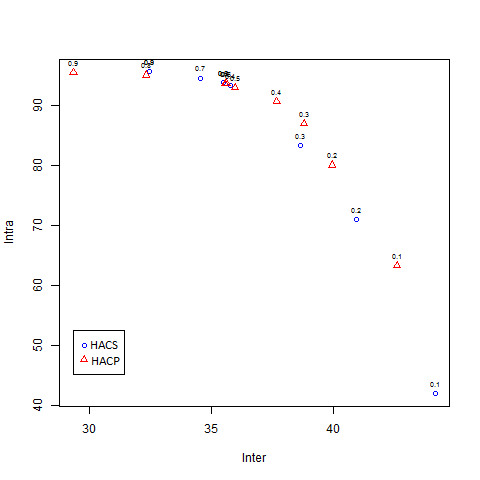
\includegraphics[width=0.5\linewidth]{img/alg1_vs_alg5.png}&
			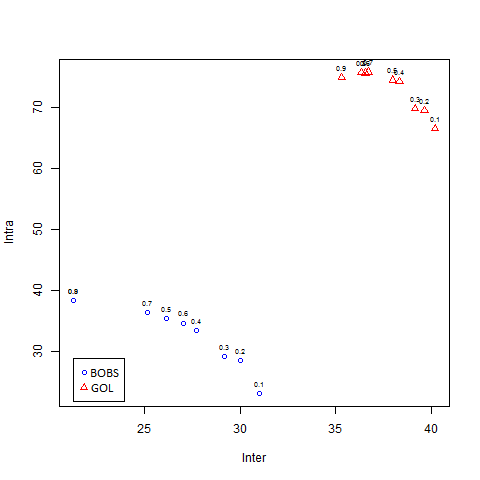
\includegraphics[width=0.5\linewidth]{img/alg2_vs_alg7.png}\\
			$alg1$ vs $alg5$ & $alg2$ vs $alg7$\\
	\end{tabular}
	\caption{}
	\label{res:inter_intra}
\end{figure}

\subsubsection{Búsqueda de autores}
En la tabla \ref{tabla:comp2} se tiene los porcentajes de deterioro de cada solución para la búsqueda de autores que escribieron artículos de tópicos similares que están afiliados a distintas universidades. Se observa que en este caso, a diferencia de la búsqueda de artículos, el algoritmo tabú no halló una mejor solución.

En PAC no hubo una diferencia considerable entre las estrategias de producción $C-HAC$ e $Inter-Intra C-HAC$. Igualmente estos algoritmos jerárquicos siguen demostrando que obtienen una mejor solución que $BOBO$. En cuanto a la etapa de selección, cuando la producción de paquetes se realizó con $BOBO$ no se detectó una mejora con la estrategia con la selección proporcional propuesta en este trabajo. Al igual a lo ocurrido en la búsqueda de artículos, el algoritmo goloso generó para todos los gammas una solución mejor que $BOBO$. En cuanto a la búsqueda tabú, a partir de las soluciones iniciales del algoritmo $alg3$ encontró soluciones mejores promedediando una mejora al rededor del $30\%$. Así como también encontró mejores soluciones para $alg5$ y $alg7$

\begin{table}[H]
\begin{center}
\begin{tabular}{|c|c|c|c|c|c|c|c|c|}
\hline
$\gamma$&$alg1$&$alg2$&$alg3$&$alg4$&$alg5$&$alg6$&$alg7$&$alg8$ \\ \hline
0.1 & -0.33 & -21.59 & -26.05 & -1.74 & -0.13 & 0.00 & -0.61 & 0.00 \\
0.2 & -0.63 & -27.46 & -29.71 & -0.52 & -0.36 & 0.00 & -1.10 & -0.25 \\
0.3 & -0.44 & -30.57 & -32.47 & -0.20 & -0.53 & 0.00 & -1.50 & -0.34 \\
0.4 & -0.25 & -32.63 & -34.29 & -0.32 & -0.25 & 0.00 & -1.88 & -0.73 \\
0.5 & -0.22 & -34.42 & -35.84 & -0.04 & 0.00 & 0.00 & -2.15 & -0.79 \\
0.6 & -0.18 & -35.86 & -37.05 & -2.01 & 0.00 & 0.00 & -2.45 & -1.39 \\
0.7 & 0.00 & -37.10 & -37.93 & -1.71 & -0.12 & 0.00 & -2.59 & -0.96 \\ 
0.8 & 0.00 & -38.19 & -38.70 & -1.44 & -0.08 & 0.00 & -2.72 & -1.20 \\
0.9 & -0.03 & -39.15 & -39.38 & -1.21 & -0.10 & 0.00 & -3.35 & -1.72 \\ \hline 
\end{tabular}
\caption{Comparación de calidad de soluciones entre algoritmos} 
\label{tabla:comp2}
\end{center}
\end{table}

En la figura \ref{res:aut_alg1_vs_alg5_vs_alg7} de la izquierda se visualiza que los valores inter e intra de las soluciones provistas por el algoritmo $alg2$ para todos los $\gamma$ son significativamente inferiores a las soluciones de los algoritmos $alg1$, $alg5$ y $alg7$. También se observa una pronunciada curva que se genera por el $\gamma$. A la derecha de la misma figura se distingue que las soluciones del algoritmo $alg5$ son más dispersas en la parte inter y están más concentradas en la parte intra que las soluciones del algoritmo $alg1$. En las soluciones del algoritmo $alg5$ la variación entre el mínimo inter y el máximo es $2.12\%$ y para el intra de $0.63\%$ mientras que para $alg1$ la variación es de $0.7\%$ para el inter y de $1.46\%$ para el intra.
\begin{figure}[H]
	\centering
	\begin{tabular}{cc}
			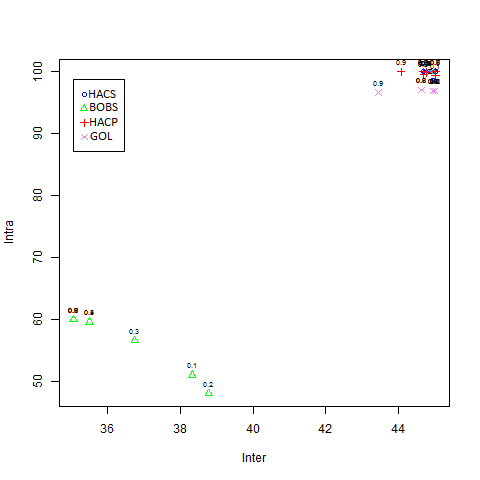
\includegraphics[width=0.5\linewidth]{img/aut-alg1-alg2-alg5-alg7.png}&
			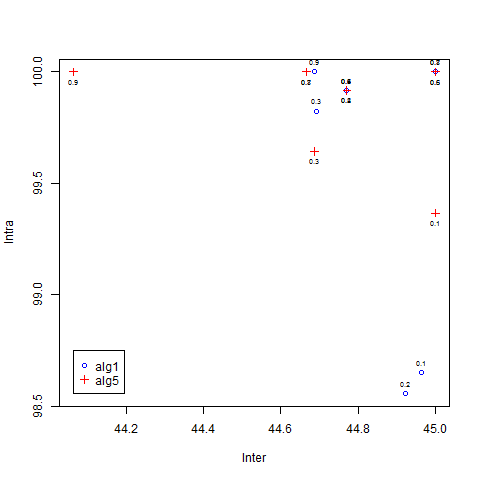
\includegraphics[width=0.5\linewidth]{img/aut-alg1-alg5.png}\\
	\end{tabular}
	\caption{}
	\label{res:aut_alg1_vs_alg5_vs_alg7}
\end{figure}


En la figura \ref{res:aut-alg-6} de la solución generada por el algoritmo $alg6$ para $\gamma = 0.1$, se tienen las siguientes observaciones:
\begin{enumerate}
	\item Todos los paquetes contienen autores que pertenecen a los mismos tópicos. 
	\item No existe un tópico que este presente en más de un paquete.
	\item Todos los paquetes utilizan el máximo del presupuesto.
\end{enumerate}
Por (1) y (2) la calidad intra e inter paquete es máxima respectivamente. Con (3) se cumple que la solución obtenida es la de máxima calidad para todo $\gamma$. Para todas las búsquedas realizadas, las soluciones que se obtuvieron cumplían con las observaciones mencionadas.

\begin{figure}[H]
  \centering
    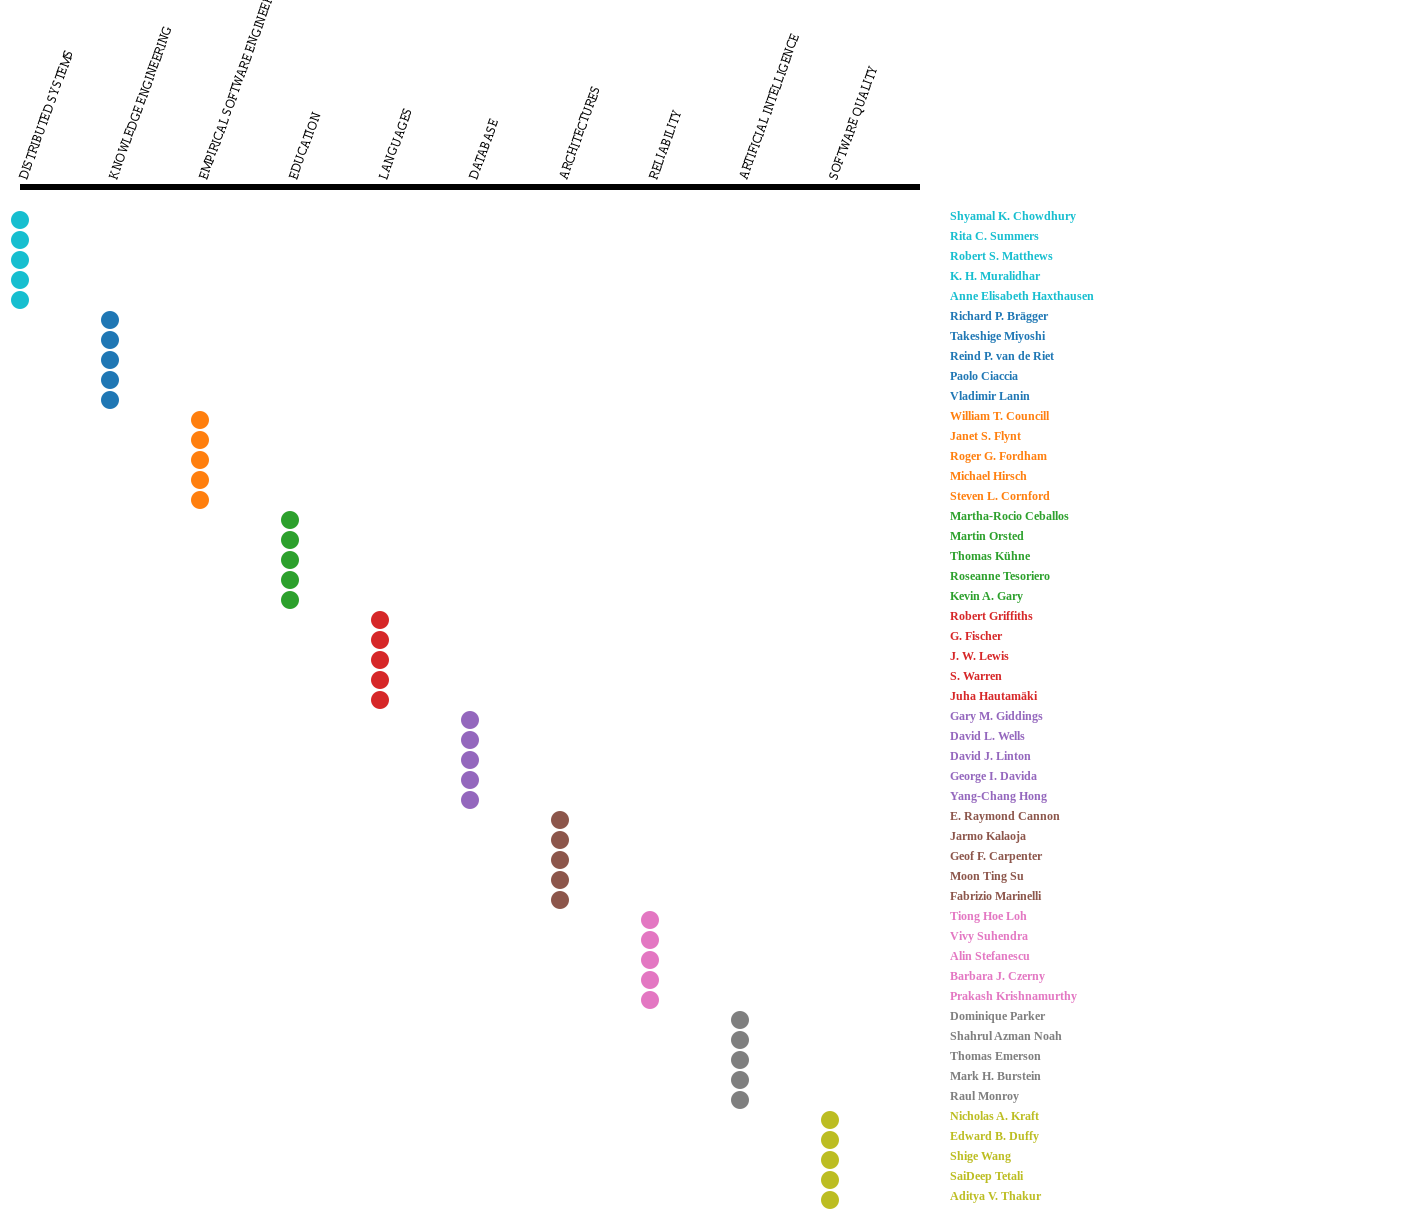
\includegraphics[width=1\textwidth]{img/aut-alg-6.png}
  \caption{}
  \label{res:aut-alg-6}
\end{figure}



\subsubsection{Búsqueda de universidades}
En este escenario lo que más se destaca de la tabla \ref{tabla:comp3} es el comportamiento del algoritmo $alg1$ que generó una mejor solución para los valores de $\gamma$ $0.1$ y $0.2$ y para el resto de los valores mayores la solución provista empeora en comparación al algoritmo $alg5$ y la brecha aumenta a medida que aumenta el $\gamma$. 

Por otro lado la función objetivo de las soluciones provista por los algoritmos $alg2$, $alg3$ y $alg7$ se encuentran muy alejadas de las soluciones provistas por los jerárquicos. En el caso del algoritmo goloso $alg7$ las soluciones mejoran con respecto a los algoritmos $alg2$ y $alg3$ cuando el valor de $\gamma$ disminuye.

En este escenario la búsqueda tabú mejoró las soluciones iniciales del BOBO y del algoritmo goloso considerablemente, pero no así con los algoritmos jerárquicos. 
\begin{table}[H]
\begin{center}
\begin{tabular}{|c|c|c|c|c|c|c|c|c|}
\hline
$\gamma$&$alg1$&$alg2$&$alg3$&$alg4$&$alg5$&$alg6$&$alg7$&$alg8$ \\ \hline
0.1 & 0.00 & -30.89 & -31.26 & -15.05 & -1.39 & -1.33 & -10.97 & -9.73 \\
0.2 & 0.00 & -40.35 & -40.16 & -22.09 & -1.72 & -1.07 & -22.83 & -20.42 \\
0.3 & -2.22 & -50.85 & -49.98 & -27.01 & -2.37 & 0.00 & -36.06 & -28.55 \\
0.4 & -5.72 & -60.65 & -58.96 & -33.76 & -1.36 & 0.00 & -48.44 & -30.38 \\
0.5 & -8.59 & -69.76 & -67.66 & -31.46 & -1.92 & 0.00 & -60.18 & -34.32 \\
0.6 & -12.09 & -77.50 & -74.71 & -33.85 & -2.53 & 0.00 & -70.16 & -35.80 \\
0.7 & -12.59 & -82.97 & -80.09 & -31.52 & 0.00 & 0.00 & -78.04 & -29.36 \\
0.8 & -15.52 & -88.12 & -84.93 & -32.90 & 0.00 & 0.00 & -85.63 & -36.34 \\
0.9 & -17.46 & -88.10 & -87.79 & -31.16 & 0.00 & 0.00 & -92.13 & -28.26 \\
 \hline 
\end{tabular}
\caption{Comparación de calidad de soluciones entre algoritmos} 
\label{tabla:comp3}
\end{center}
\end{table}

\subsection{Búsqueda de atracciones turísticas}\label{res:busAtracciones}
En las búsquedas realizadas sobre la base de datos de atracciones turísticas las soluciones obtenidas a partir de las modificaciones propuestas en este trabajo de los algoritmos PAC mejoran a los originales en todos. Es para destacar que en en este escenario el algoritmo goloso supera a $alg1$. La búsqueda tabú consiguió mejores resultados para los algoritmos PAC, pero no así para el algoritmo goloso.

\begin{table}[H]
\begin{center}
\begin{tabular}{|c|c|c|c|c|c|c|c|c|}
\hline
$\gamma$&$alg1$&$alg2$&$alg3$&$alg4$&$alg5$&$alg6$&$alg7$&$alg8$ \\ \hline
0.1 & -6.49 & -22.89 & -22.30 & -9.99 & -0.05 & 0.00 & -0.52 & -0.52 \\
0.2 & -13.50 & -27.60 & -26.57 & -16.51 & -0.09 & 0.00 & -1.09 & -1.09 \\
0.3 & -21.10 & -32.76 & -29.73 & -20.58 & -0.15 & 0.00 & -1.70 & -1.70 \\
0.4 & -29.38 & -36.68 & -33.51 & -25.10 & -0.20 & 0.00 & -2.37 & -2.37 \\
0.5 & -38.43 & -42.05 & -38.44 & -30.94 & -0.27 & 0.00 & -3.10 & -3.10 \\
0.6 & -48.35 & -47.73 & -43.86 & -34.75 & -0.34 & 0.00 & -3.90 & -3.90 \\
0.7 & -59.29 & -51.47 & -50.54 & -43.46 & -0.41 & 0.00 & -4.78 & -4.78 \\
0.8 & -71.36 & -57.07 & -56.14 & -45.61 & 0.00 & 0.00 & -5.62 & -5.62 \\
0.9 & -84.97 & -60.59 & -59.81 & -44.04 & 0.00 & 0.00 & -7.33 & -7.33 \\
\hline 
\end{tabular}
\caption{Comparación de calidad de soluciones entre algoritmos} 
\label{tabla:comp4}
\end{center}
\end{table}

En la figura \ref{res:cit_bobo_diff} se visualiza el porcentaje de mejora del algoritmo $alg3$ para cada valor de $\gamma$ con respecto a $alg2$. En promedio el porcentaje de mejora es de $3.5\%$ y la mayor diferencia se da para los valores de $\gamma$ $0.3$, $0.4$ y $0.5$
y en los extremos la diferencia disminuye.
\begin{figure}[H]
  \centering
    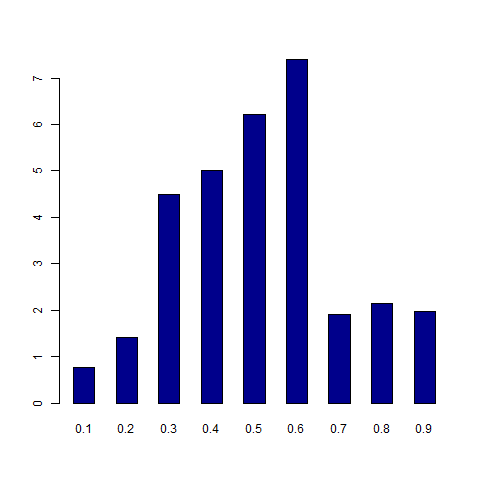
\includegraphics[width=1\textwidth]{img/cit_bobo_diff.png}
  \caption{}
  \label{res:cit_bobo_diff}
\end{figure}
